\section{Problema 2}

\subsection{Enunciado}
El enunciado nos plantea una situación en donde tenemos $n$ localidades conectadas entre si, mediante uno o más enlaces telefónicos. La empresa desea que la conectividad entre todas las ciudades nunca se pierda, por lo que está interesada en invertir en cableado subterraneo indestructible. El precio de conectar las distintas localidades varía según las mismas, por lo que la empresa nos pide que hallemos la forma de conectar todas las ciudades y que ninguna quede incomunicada, de forma de que la inversión en éste nuevo cableado subterraneo sea mínima.

\subsection{Soluci\'on}
l presentarnos éste problema, inmediatamente pensamos que era posible reprentarlo mediante un problema de grafos. El mismo representaría todo la red de conectividad de la empresa telefónica, los vértices del mismo representarían las localidades y las aristas entre los distintos nodos representarían el costo del cableado subterraneo entre las ciudades que uniera la misma.
Dicho ésto, el problema se reducía, entonces, a hallar un grafo cuyas aristas permitan ir de una ciudad a cualquier otra del grafo, y además, a que esas aristas tengan un costo mínimo de construcción. En otras palabras, necesitamos un algoritmo que nos calcule, dado un grafo cualquiera, el arbol generador mínimo (AGM). El agm es un grafo que contiene los mismo vértices que el original, pero sólo contiene v-2 aristas (siendo v la cantidad de vértices), que unen todo el grafo y cuyo peso total es mínimo.
Para el problema, hemos implementado una clase propia de Grafo, representanda por una lista de adyacencia, y utilizado el conocido y demostrado Algoritmo de Prim para generar el AGM. El mismo consiste en, dado un grafo cualquiera, agarrar un vértice del mismo al azar, y agregarlo al AGM (que originalmente no tenía ningún vértice ni aristas). Luego, agregamos al grafo la arista de menor peso que conecte al vértice recién insertado con un vértice que no esté en el agm. Para ello, agregamos todas las aristas del vértice en una cola de prioridad, y vamos desencolando hasta que encontremos una arista que tenga un extremo en el agm y otro no (es decir, tengo un sólo vértice en el árbol). Una vez que encontramos dicha arista, agregamos el vértice que no estaba al AGM y también la arista. El proceso debe ser repetido, de la misma forma, con todos los vértices del grafo, es decir, hasta que la cantidad de vértices que hay en el árbol sea la misma que había en el grafo original. Ésta es la forma en que se describe el algoritmo de prim y la forma en que actúa nuestro algoritmo, por lo que podemos decir que la implementación realizada se corresponde con dicho algorítmo.

\subsection{Pseudoc\'odigo}
En código del ejercicio básicamente hace una cosa: lee el archivo de entrada, y procesa las lineas y va creando las distintas instancias del ejercicio. La lógica del problema está toda delegada en la clase Grafo, que es la que se encarga de modelar las localidades y sus enlaces (el grafo en sí), y luego, una vez modelado, de crear el propio AGM. El agm está implementado a partir del algoritmo de prim, que busca para cada vertice nuevo agregado, la arista de menor peso que lo conecte con un vertice que no esté en el grafo y la agrega.
La lógica del ejercicio podría dividirse, de acuerdo a lo recién mencionado, de la siguiente manera:

\begin{verbatim}
Grafo CrearGrafoAPartirInstancia():
	Grafo g;
	para cada enlace de la instancia:
		agrego el vertice 1
		agrego el vertice 2
		agrego la arista entre v1 y v2
	devuelvo el grafo 
\end{verbatim}

\begin{verbatim}
Grafo getAgm():
	Grafo agm;
	agrego un vertice al azar del grafo al agm
	marco el vertice agregado como visitado
	agrego las aristas del vertice visitado a la cola de prioridad
	para cada vertice en grafo:
		obtengoLaAristaDeMenorPesoDeLaCola()
		miro los dos vertices de la arista
		si alguno no fue visitado:
			agrego la arista minima al agm
			marco el vertice como visitado
			agrego las aristas del vertice a la cola de prioridad
	devuelvo el agm
\end{verbatim}

\subsection{Analisís de complejidad}	
Para averiguar cuanta gente hay en todo el edificio tenemos que recorrer todo el vector 'pisos' e ir sumando la cantidad de gente en cada piso. Eso nos cuesto O(n) donde n es la cantidad de pisos. Luego hacemos una búsqueda binaria sobre la cantidad total de gente que mediante la función sePuedeLevantar busca el máximo de gente que es posible cargar. La complejidad de la búsqueda binaria es de O(log cantGente) (esto es sabido, porque ya lo vimos en algoritmos y estructura de datos 2) y la complejidad de la función sePuedeLevantar en el peor caso (sería cuando tiene que irse hasta el último piso para poder levantar la cantidad de gente solicitada y tiene energía suficiente para levantarlos a todos) es de: \\
	O( $\sum\limits_{i=0}^{n} { ( \lceil (pisos[i]/capacidad) \rceil  + i}$ ) ) \\
Esto es porque por cada piso al que voy tengo que ir tantas veces tal que levante el total de gente de ese piso (eso es $\lceil$pisos[i]/capacidad$\rceil$) y luego en caso que me haya sobrado espacio voy recorriendo todos los pisos inferiores para llenar la capacidad restante.
Finalmente la complejidad total del ejercicio nos queda:\\
O( n + Log(g) * $\sum\limits_{i=0}^{n} { ( \lceil (pisos[i]/capacidad) \rceil  + i ) }$ ) \\
Donde n es la cantidad total de pisos y g la cantidad total de gente en todo el edificio.
\subsection{Tests y Gráficos}
Con respecto a los tests realizados, los mismos no se hicieron en cuanto a la complejidad (ya que al utilizar estructuras primitivas de java, podemos asegurar que la complejidad de cada una de sus operaciones es la que aparece en la documentación de ellas y por tanto, es la que detallamos en el apartado anterior), sino en cuanto a la cantidad de ciclos que realiza cada solución (más precisamente, la creación del árbol generador mínimo) para distintas instancias, de acuerdo a la cantidad de vértices (localidades) y aristas (enlaces) que posee cada una.
Como podemos apreciar en los siguientes gráficos, la cantidad de ciclos, para grafos en donde la cantidad de aristas es la misma, es directamente proporcional a la cantidad de vértices que contenga el mismo (figura 1). Es cierto que en algunos casos ésto no se cumple pero, en el caso promedio, a más cantidad de vértices, con igual cantidad de aristas, más ciclos tendrá que hacer nuestro algoritmo para encontrar el AGM válido. Los casos extremos serían aquellos en donde las aristas se insertan ordenados de la misma forma que los leerá nuestro algoritmo, donde la cantidad de ciclos se corresponde con la cantidad de vértices. Por el contrario, el peor caso se da cuando hay muchas aristas de 2 vértices que ya fueron visitados, de menor peso de aquellas que contengan 1 vértice visitado y otro sin visitar. De ésta forma, el algoritmo hará tantos ciclos como aristas tenga el vértice para, recién en la último, procesar el vértice y agregarlo al AGM.
\begin {center}
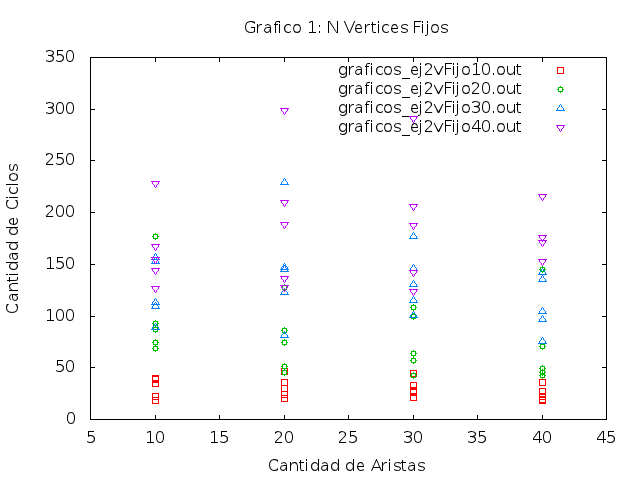
\includegraphics[width=8cm]{./graficos/grafico_vfijo.png}
% grafico.eps: 0x0 pixel, 300dpi, 0.00x0.00 cm, bb=50 50 410 302
\end {center} 
Por otro lado, y con respecto a la figura 2, donde la cantidad de aristas está fijo, vemos que la cantidad de ciclos que se llevan a cabo es netamente aleatorio, ya que, de acuerdo a cómo estén distribuidas las distintas aristas y sus pesos, es posible crear el AGM en n pasos, siendo n la cantida de vértices, o bien, en n x e(n), siendo e(n) la cantidad de aristas de n. El primer caso se daría sólo cuando el grafo que analizamos posee aristas minimas sin descubrir en todos los pasos, mientras que el peor caso, que sería el de recorrer todas las aristas del vértice, es el mismo que analizamos en el párrafo anterior.
\begin {center}
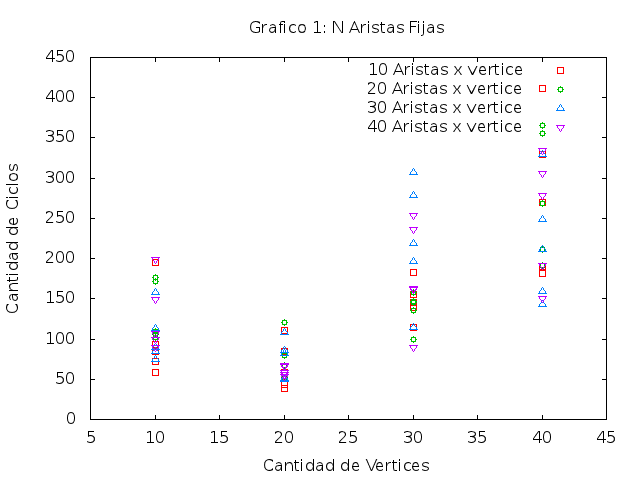
\includegraphics[width=8cm]{./graficos/grafico_efijo.png}
% grafico.eps: 0x0 pixel, 300dpi, 0.00x0.00 cm, bb=50 50 410 302
\end {center} 


\subsection{Conclusiones}
A partir del problema dado, hemos podido modelar a partir de la teoría de grafos. De ésta forma, e interpretando qué es lo que nos pide el enunciado, hemos podido resolver el problema a partir de un algoritmo que es conocido y, de esa forma, podemos afirmar que estamos dando la solución correcta. 
En ésta caso, modelamos nuestras localidades y los distintos precios que costaban unirlas a partir de un grafo conexo, no dirigido. Para éstos grafos, es posible hallar un grafo de peso mínimo que conecte todas las ciudades, conocido también como árbol generador mínimo (agm). Precisamente, ésto es lo que nos pedía el enunciado: hallar la forma de conectar todas las ciudades de forma tal que el coste de unirlas todas sea mínimo. Con nuestro planteo, logramos responder dicho problema, teniendo en cuenta, además, la complejidad pedida para resolverlo. La misma fue lograda no sólo implementando un algoritmo conocido, como es el de prim, sino que se fue cuidadoso a la hora de elegir las estructuras de datos utilizadas para mantenernos dentro de la cota estipulada.
